\chapter{Literature Review}

\section{Spatial Database}
Spatial database is a database designed to store and process data with spatial data types such as point, line, or region contained in Geographic Information System (GIS). Spatial data can be utilized on a two dimensional appearance as the appearance of the earth's surface, or the appearance of three dimensions, such as modeling the human brain, the protein molecule chains, etc. After the systems of relational database developed, the system of other databases become developed then, one of it is the spatial database. Characteristics of spatial database needed is a system that is able to accommodate simple geometric objects data with a huge amount to accommodate as 100,000 polygons.

Spatial database system is gaining popularity in recent years, especially at a "Symposium on Large Spatial Databases (SSD)" held biennially since 1898 associated with the database that stores the object in space as a supporter of space images \cite{okabe2009spatial}.
\subsection{Data Representation}
As mentioned previously, spatial data can be represented by a point, line, or region. For example, a city can be modeled as a set of points that describe a large geographical area. A line usually used to represent the connections in space such as roads, rivers, telephone cables, electricity, etc. An object representing the area or region that has a limit in two-dimensional space, such as the state, lakes, etc. Figure 2.1 is a basic representation of an image on a spatial database, which is the point, line, and area.
\begin{figure}[h!]
	\centering
	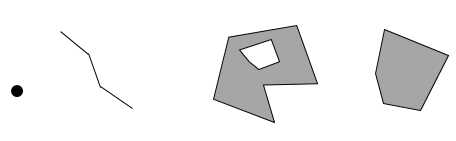
\includegraphics[scale=0.5]{figure1.png}
	\caption{Three basic spatial representations: points, lines, areas}
	\label{fig:figure1}
\end{figure}

Spatial objects relate to each other can be described by the form of partitions or networks as shown in Figure 2.2 below. 

\begin{figure}[h!]
	\centering
	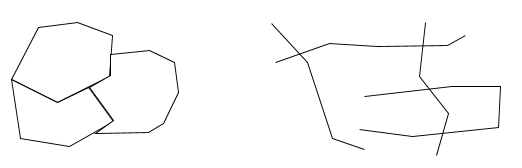
\includegraphics[scale=0.7]{figure2.png}
	\caption{Partitions and networks}
	\label{fig:figure2}
\end{figure}

A partition can be described by a group of separate region. The liaison between the regions is the regions’ equally boundary. For example, the partition can be used to represent a thematic map. A network can be illustrated by the graph that are connected in a field where each object point considered as nodes and lines as the geometric shapes of the edges. This network forms can be used to represent roads, rivers, public transportation, or electricity cable lines \cite{guting1994introduction}.


\section{Routing System}
Routing System is a system that provides driving directions or routes that can be taken by a moving object in order to reach a location of the destination. This system is often referred to the navigation system. Modern navigation systems now have integrated between the position of the object, sensors, computing, and communications between the hardware and software to support the facilities in humans, vehicles, and other moving objects. In addition, modern navigation systems also consider the geographical location coordinates distance accuracy, speed, and altitude of the moving object. The navigation system is widely used in outdoor data. But along with the times, this system is also applied to the indoor data.

\subsection{Outdoor Routing}
Outdoor routing technology is now highly developed. Figure 2.3 describes the flow of information on outdoor navigation systems.

\begin{figure}[h!]
	\centering
	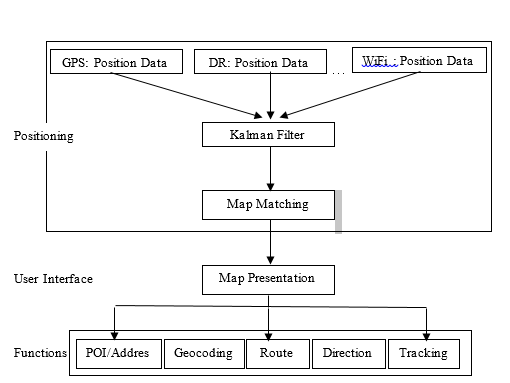
\includegraphics[scale=0.7]{figure3.png}
	\caption{The information flow on outdoor navigation systems}
	\label{fig:figure3}
\end{figure}

From Figure 2.3, the user's position is determined by: (a) obtaining position data through geo-positioning sensor and (b) applying the map matching algorithm using position data obtained. These steps are general steps to improve the accuracy, availability, and reliability of outdoor navigation system by using more than one geo-positioning sensor in which each of the position data can be filtered using a Kalman filter to find the best position estimation. Furthermore, the position data that has been filtered out will be input to the map matching algorithm that uses a database map for traveling the area, which contains spatial and non-spatial to find: (a) roads / pavements where users are located and (b) the location right of user in the segment.

When the user's location is known, the locations will be marked in the map and displayed to the user. At this stage, the system is currently tracking, and users have the option to search for POIs or a request for an optimal route between the pair of addresses. The system uses a search using the shortest or fastest route criteria\cite{karimi2011universal}. Figure 2.4 is an example of outdoor routing system implementation.

\begin{figure}[h!]
	\centering
	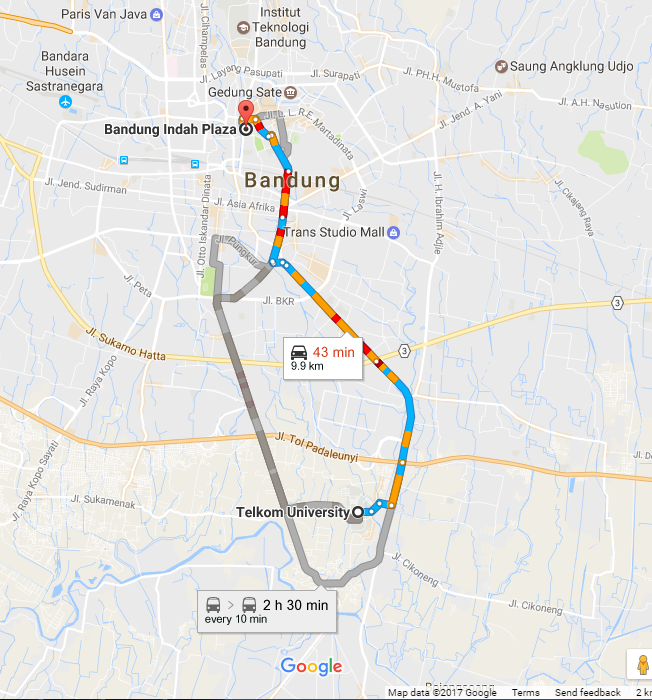
\includegraphics[scale=0.7]{figure4a.png}
	\caption{Examples of outdoor routing implementation}
	\label{fig:figure4}
\end{figure}

\subsection{Indoor Routing}
Indoor routing is a routing system implementation in the room or building. By using spatial data, each space can be accurately identified. There are various kinds of elements in indoor spaces such as rooms, doors, corridors, floors, stairs, elevators, and the road connection between buildings. Indoor spaces are represented by undirected graph with nodes and edges. The concept of modeling the indoor spaces can be summarized in Table 2.1.

\begin{table}[h!]
	\centering
	\caption{The concept of indoor spaces modeling} %\ref{fig:figure9}}
	\label{indoor-concept-table}
	\begin{tabular}{|l|l|l}
		\cline{1-2}
		\textbf{Domain Concept} & \textbf{Modeling Concept}   &  \\ \cline{1-2}
		Room		&	A cell &  \\ \cline{1-2}
		Door		&	An edge  &  \\ \cline{1-2}
		Corridor	&	One or more cells with one or more edges &  \\ \cline{1-2}
		Stair		&	One or more cells with one or more edges &  \\ \cline{1-2}
		Elevator	&	One cell with several edges &  \\ \cline{1-2}
		Pathway		&	One or more cells with several edges &  \\ \cline{1-2}
	\end{tabular}
\end{table}

As an illustration, Figure 2.5 is a graph modeling the indoor spaces delineated by one level.

\begin{figure}[h!]
	\centering
	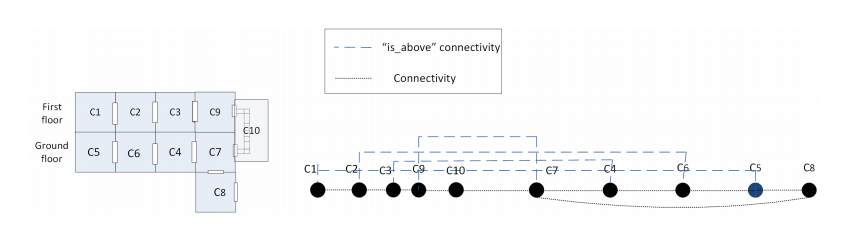
\includegraphics[scale=0.6]{figure5a.png}
	\caption{Modeling indoor spaces with a graph of the level }
	\label{fig:figure5}
\end{figure}

From the illustration, it can be seen that C10, C9, C8, C7, C4, C6, C5, C3, C2 and C1 are connected where C10 is the ladder that connects the ground floor and the first floor. Given this concept, it can be concluded that:
\begin{enumerate}
	\item An indoor space is a connected undirected graph (Cells, Edges), where Cells = {C1, C2, ..., Cn} is a set of cells, and Edges = {E1, E2, . . . , Em} is set of edges, each of which is a set of two cells, that is, each edge connects two distinct cells. 
	\item (Adjacent Nodes) Let G = (N,C) be a graph, and two Nodes n1,n2 $\in$ N of G are adjacent if: $\exists$ n1,n2 are connected.
	\item (Multidimensional Connectivity Graph) Given a set of cells Ci , Cj , Cf , Cl in the ground floor and a set of cells Cx, Cy,Cr, Ct the multidimensional connectivity graph refers to the multiple edges that connect the single floor cells and the above cells in the multi-floor space\cite{alamri2014adjacency}.
\end{enumerate}	 

\section{Shortest Path Algorithms}
There are several algorithms that the accuration and time complexity have been tested to calculate the shortest distance between nodes on a graph, like Djikstra algorithm, Floyd-Warshall, Bellman-Ford, and Genetic Algorithm (GA). Here are the description of each algorithms.

\subsection{Dijkstra's Algorithm}
For each vertex within a graph we assign a label that determines the minimal length from the starting point $s$ to other vertices $v$ of the graph. In a computer we can do it by declaring an array $d[]$. The algorithm works sequentially, and in each step it tries to decrease the value of the label of the vertices. The algorithm stops when all vertices have been visited. The label at the starting point $s$ is equal to zero $(d[s] = 0)$; however, labels in other vertices $v$ are equal to infinity $(d[v] =\infty)$, which means that the length from the starting point $s$ to other vertices is unknown. In a computer we can just use a very big number in order to represent infinity. In addition, for each vertex $v$ we have to identify whether it has been visited or not. In order to do that, we declare an array of Boolean type called $u[v]$, where initially, all vertices are assigned as unvisited $(u[v] = false)$. The Dijkstra’s algorithm consists of $n$ iterations. If all vertices have been visited, then the algorithm finishes. Otherwise, from the list of unvisited vertices we have to choose the vertex which has the minimum (smallest) value at its label (At the beginning, we will choose a starting point $s$). After that, we will consider all neighbors of this vertex (Neighbors of a vertex are those vertices that have common edges with the initial vertex). For each unvisited neighbor we will consider a new length, which is equal to the sum of the label’s value at the initial vertex $v (d[v])$ and the length of edge $l$ that connects them. If the resulting value is less than the value at the label, then we have to change the value in that label with the newly obtained value\cite{magzhan2013review}.
\begin{equation}\label{finding-minimum-neighbour-in-dijkstra}
	d [ neighbors ] = min ( d [ neighbors ] , d[ v ] + l )
\end{equation}

After considering all of the neighbors, we will assign the initial vertex as visited $(u[v] = true)$. After repeating this step $n$ times, all vertices of the graph will be visited and the algorithm finishes or terminates. The vertices that are not connected with the starting point will remain by being assigned to infinity. In order to restore the shortest path from the starting point to other vertices, we need to identify array $p []$, where for each vertex, where $v \neq s$, we will store the number of vertex $p[v]$, which penultimate vertices in the shortest path. In other words, a complete path from $s$ to $v$ is equal to the following statement.

\begin{equation}\label{finding-path-in-dijkstra}
P = ( s , … , p [ p [ p [ v ] ] ] , p [ p [ v ] ] , p [ v ] , v )	
\end{equation}

Figure \ref{fig:figure6} is an implementation of Dijkstra's algorithm using the Java programming language.

\begin{figure}[h!]
	\centering
	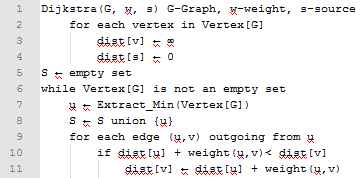
\includegraphics[scale=1]{figure6.png}
	\caption{Dijkstra's algorithm pseudocode}
	\label{fig:figure6}
\end{figure}

\subsection{Floyd-Warshall Algorithm}
Consider the graph $G$, where vertices were numbered from 1 to $n$. The notation dijk means the shortest path from $i$ to $j$, which also passes through vertex $k$. Obviously if there is exists edge between vertices $i$ and $j$ it will be equal to $d_{ij0}$, otherwise it can assigned as infinity. However, for other values of dijk there can be two choices: (1) If the shortest path from $i$ to $j$ does not pass through the vertex $k$ then value of $d_{ijk}$ will be equal to $d_{ijk- 1}$. (2) If the shortest path from $i$ to $j$ passes through the vertex $k$ then first it goes from $i$ to $k$, after that goes from $k$ to $j$. In this case the value of $d_{ijk}$ will be equal to $d_{ikk-1} + d_{kjk-1}$. And in order to determine the shortest path we just need to find the minimum of these two statements:


\begin{equation}\label{length-between-i-j}
	d_{ij0} = the \; length \; of \; edge \; between \; vertices \; i \; and \; j
\end{equation}

\begin{equation}\label{length-between-i-j}
	d_{ijk} = min (d_{ijk-1}, d_{ikk-1} + d_{kjk-1})	
\end{equation}

\begin{figure}[h!]
	\centering
	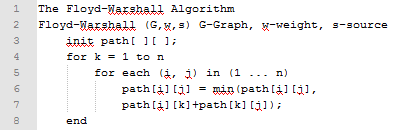
\includegraphics[scale=1]{figure7.png}
	\caption{Floyd-Warshall algorithm pseudocode}
	\label{fig:figure7}
\end{figure}
\vspace{40mm}
\subsection{Bellman-Ford Algorithm}
In comparison to Dijkstra’s algorithm, the Bellman-Ford algorithm admits or acknowledges the edges with negative weights. That is why, a graph can contain cycles of negative weights, which will generate numerous number of paths from the starting point to the final destination, where each cycle will minimize the length of the shortest path. Taking into consideration this fact, let’s assume that our graph does not contain cycles with negative weights. The array $d[]$ will store the minimal length from the starting point $s$ to other vertices. The algorithm consists of several phases, where in each phase it needs to minimize the value of all edges by replacing $d[b]$ to following statement $d[a] + c; a$ and $b$ are vertices of the graph, and $c$ is the corresponding edge that connects them. And in order to calculate the length of all shortest paths in a graph it requires $n – 1$ phases, but for those vertices of a graph that are unreachable, the value of elements of the array will remain by being assigned to infinity \cite{magzhan2013review}.

Figure 2.9 is the Bellman-Ford algorithm implementation using the Java programming language.
 
\begin{figure}[h!]
	\centering
	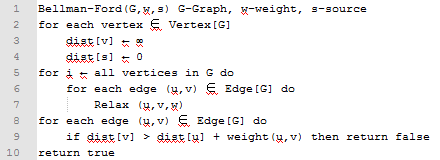
\includegraphics[scale=1]{figure8.png}
	\caption{Bellman-Ford algorithm pseudocode}
	\label{fig:figure8}
\end{figure}

\subsection{A* Algorithm}
The A* (called as ‘A-star’) (Cvetanovic and Nofsinger 1990) is like other graph searching algorithms in that it can potentially search a huge area of the map. It’s like Dijkstra’s algorithm in that it can be used to find a shortest path. It’s like breadth first search (BFS) in that it can use a heuristic to guide itself. In the simple case, it is as fast as BFS. Since in the worst case breadth-first search has to consider all paths to all possible nodes the time complexity of breadth-first search is increased depending on the number of nodes and edges in the graph \cite{sathyaraj2008multiple}.

This heuristic search ranks each node by an estimate of the best route that goes through that node. The typical formula is expressed as:

\begin{equation}\label{A-star-heuristic}
f(n) = g(n) + h(n)	
\end{equation}

where $f(n)$ is the score assigned to node $n$, this is the estimate of the best solution that goes through $n, g(n)$ is the actual cheapest cost of arriving at from the start node to $n$ and $h(n)$ is the heuristic estimate of the cost to the goal from $n$ (Fig. 7).

\begin{figure}[h!]
	\centering
	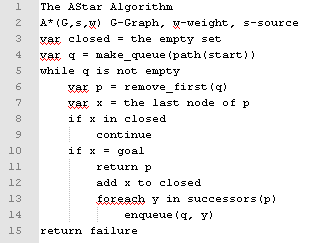
\includegraphics[scale=1]{figure9.png}
	\caption{A* algorithm pseudocode}
	\label{fig:figure9}
\end{figure}

\section{Three Dimensional Spaces}
If a rubber ball thrown vertically from the floor, the ball will have a unique coordinate axes. Figure 2.10 is an illustration of the movement of a rubber ball thrown vertically. For example, a spherical coordinate to the axis of the two-dimensional space (in this case on the floor) is (5, 4) and the high ball as reflected by the floor is 2.5 cm, then the spherical coordinates into (5.4, 2.5). Each position of the vertical movement of the ball is a unique three dimensional space coordinates. 

\begin{figure}[h!]
	\centering
	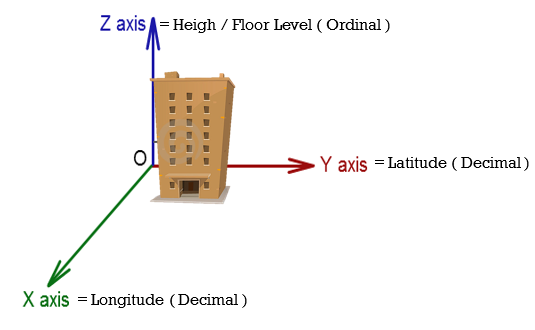
\includegraphics[scale=1]{figure10.png}
	\caption{Illustration of Rubber Ball Movement}
	\label{fig:figure10}
\end{figure}

\section{Distance between Two Points}
Measuring the distance between two points on a three dimensional space can be illustrated in Figure \ref{fig:figure11} below. If there is a power outlet in an area of a wall in a room and there is an electric iron on the table, how many minimum length of electric cable that needed to connect the iron to a power outlet? 

\begin{figure}[h!]
	\centering
	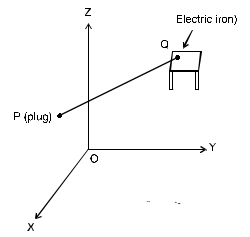
\includegraphics[scale=1]{figure11.png}
	\caption{Ilustration of distance between two points on a Three Dimensional Spaces}
	\label{fig:figure11}
\end{figure}

If the coordinates of the point $P$ is $(x_1, y_1, z_1)$ and point Q is $(x_2, y_2, z_2)$, then the distance between point $P$ and point $Q$ or $|PQ|$ can be determined by using the following formula:


\begin{equation}\label{distance-between-2-points}
|PQ|= \sqrt{(x_2 - x_1)^2 + (y_2 - y_1)^2 + (z_2 - z_1)^2}
\end{equation}

Thus, it can be seen that the general equation of distance point $P (x, y, z)$ to the center point $O (0,0,0)$ will be as follows:

\begin{equation}\label{A-star-heuristic}
|PQ|= \sqrt{(x_2 - 0)^2 + (y_2 - 0)^2 + (z_2 - 0)^2}
\end{equation}

\begin{equation}\label{A-star-heuristic}
|PQ|= \sqrt{(x_2)^2 + (y_2)^2 + (z_2)^2}
\end{equation}

In other case, such as the distance between a room in the first floor and the one in the third floor of a bilding, we can’t just use that formula to measure the distance. There is a route that we have to consider. Figure \ref{fig:figure12} shows the route wich include rooms, corridors, and stairs of a building. To measure the distance between room R1 and room R2, we have to measure the exact length of the route.

\begin{figure}[h!]
	\centering
	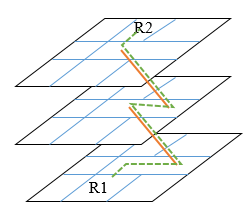
\includegraphics[scale=1]{figure12.png}
	\caption{Ilustration of distance between two rooms}
	\label{fig:figure12}
\end{figure}
\subsection{Spatial Data Distance Calculation using Haversine Formula}
The Haversine formula is an equation important in navigation, giving great-circle distances between two points on a sphere from their longitudes and latitudes. These names follow from the fact that they are customarily written in terms of the haversine function, given by $haversin (\theta) = sin^2
(\theta/2)$. The haversine formula is used to calculate the distance between two points on the Earth’s surface specified in longitude and latitude \cite{chopde2013landmark}.

\begin{equation}\label{A-star-heuristic}
d=2r sin^-1 ( \sqrt{sin^2 (\dfrac{\phi_2 - \phi_1}{2})}+cos(\phi_1)cos(\phi_2) sin^2(\dfrac{\psi_2-\psi_1}{2}))
\end{equation}

$d$ is the distance between two points with longitude and latitude $(\psi,\theta)$ and $r$ is the radius of the Earth.

\section{Summary}
This chapter is about the references that will be used in this final project. The theories and the algorithm will be implemented in building the Indoor Routing System.